\documentclass[10pt]{article}
\usepackage[margin=1 in, letterpaper]{geometry}
\usepackage{fontspec, graphicx, amsmath, amssymb, amsthm, array, physics, enumitem, cancel, multicol, float}
\usepackage[dvipsnames]{xcolor}

\setmainfont{Linux Libertine O}
\setsansfont{Linux Biolinum O}
\setmonofont{Latin Modern Mono}
\setmathrm{Latin Modern Math}
\theoremstyle{definition}
\newtheorem{theo}{\color{Maroon} Theorem}[section] 
\newtheorem{defin}[theo]{\color{Maroon} Definition}
\newtheorem{example}[theo]{\color{Maroon} Example}
\newtheorem{prob}[theo]{\color{Maroon} Problem}
% \newtheorem{example}[section]{\color{Maroon} Example}

\theoremstyle{remark}
\newtheorem*{soln}{\color{Maroon} Solution}


\newcommand{\R}{\mathbb{R}}
\newcommand{\Q}{\mathbb{Q}}
\newcommand{\Z}{\mathbb{Z}}
\newcommand{\N}{\mathbb{N}}

%%%%%%%%%%%%%%%%%%% Statistics %%%%%%%%%%%%%%%%%%%%
\newcommand{\E}[1]{\mathbb{E}\left[ #1 \right]}
\newcommand{\Prob}[1]{\mathbb{P}\left[ #1 \right]}
\newcommand{\cov}[2]{\textnormal{Cov}\left[ #1, #2 \right]}
\renewcommand{\var}[1]{\textnormal{Var}\left[ #1 \right]}
\newcommand{\Unif}{\textnormal{Unif}}
\newcommand{\Norm}{\mathcal{N}}

%%%%%%%%%%%%%%%%%%%%%%%%%%%%%%%%%%%%%%%%%%%%%%%%%%%%%%%%%%%%%%%%%%%%
\newcommand{\inserttitle}{Section 01}
\newcommand{\insertauthor}{Max Guo \& Seung Hwan An}
\newcommand{\insertcourse}{STAT 110}
%%%%%%%%%%%%%%%%%%%%%%%%%%%%%%%%%%%%%%%%%%%%%%%%%%%%%%%%%%%%%%%%%%%%

\usepackage{fancyhdr}
\setlength{\headheight}{15pt}
\pagestyle{fancy}
\fancyhf{}
\fancyhead[C]{\thepage}
\fancyhead[L]{\inserttitle}
\fancyhead[R]{\insertauthor}

%%%%%%%%%%%%%%%%%%%%%%%%%%%%%%%%%%%%%%%%%%%%%%%%%%%%%%%%%%%%%%%%%%%%

\begin{document}

{\noindent\Huge\bf  \\[0.1\baselineskip] {\inserttitle }}\\[2\baselineskip]
{{\bf \insertcourse}\\ {\textit{September 13, 2021}}} \hfill {\large \textsc{\insertauthor}}
\smallskip

\hfill \noindent \textit{Credits to Ginnie Ma and Rachel Li}

\section{Probability}

Probability is a mathematical language for quantifying uncertainty. Learning this language begins with representing events with sets.

\subsection{Events}

The \textbf{sample space} $S$ of an experiment is the set of all possible outcomes of the experiment. An event $A$ is one of these outcomes, and we say that $A$ occurred if the actual outcome is $A$.

\subsection{Set Notation}

Set theory provides the language to express and work with events.\\

\noindent
Let $A$ and $B$ be subset of some sample space $S$, that is, $A,B \subseteq S$. Then, $A^c = S \setminus A$ is the \textbf{complement} of subset $A$, and similarly $B^c = S \setminus B$.

\begin{defin} \textbf{(DeMorgan's Laws)} Fundamentals of propositional logic and Boolean algebra:
\begin{align*}
    (A\cup B)^c &= A^c \cap B^c \\
    (A\cap B)^c &= A^c \cup B^c
\end{align*}
\end{defin}

\subsection{Naive Definition of Probability}
Let $A$ be an event for an experiment with a finite sample space $S$. The naive probability of $A$ is:
\begin{align*}
    P_{naive}(A) &= \frac{\text{number of outcomes favorable to $A$}}{\text{number of outcomes in $S$}}
\end{align*}

\noindent
\textbf{Note:} This applies when there is symmetry or equally likely outcomes in a problem.

\section{Counting}

Now that we have a naive definition of probability, how do we count the number of outcomes? The following rules/strategies give us a way to count these outcomes so we can compute probabilities. Counting is also known as combinatorics.

\subsection{Multiplication Rule}
\begin{defin} \textbf{(Multiplication Rule)} Suppose that Experiment A has $a$ possible outcomes, and for each of those outcomes Experiment B has $b$ possible outcomes. Then the compound experiment has $ab$ possible outcomes, given that the number of outcomes of each experiment doesn't depend on the outcomes of the other.
\end{defin}

\begin{example} \textbf{(Jefe's or Felipe's)} You are hungry and want to eat some good food. You can choose to go to either Jefe's or Felipe's. At each of these restaurants, you can choose to order a burrito, quesadilla, or nachos. How many possibilities are there for your food order? What if you buy food twice, once in the morning and once in the afternoon, how many possibilities are there?\\

\noindent
\textbf{Note:} The order of $ab$ or $ba$ doesn't matter for the multiplication rule. In this example, you can either choose \textit{what} you want to eat first or \textit{where} you want to eat first and you will still get the same number of possibilities.\\

\noindent
\textbf{An important caveat: }If you are only interested in what foods you got that day, not the order in which you got them, how many possibilities are there? The answer is \textit{not} 36/2. It is true that because we don't care about order, possibilities like (Jefe's burrito, Felipe's nachos) are now listed twice since we count $(x,y)$ to be equivalent with $(y,x)$. However, some possibilities, like (Jefe's burrito, Jefe's burrito), onnly are listed once in the original list of $36$ ordered possibilities. So dividing 36 by two would miscount these. To find the right answer, we know that there are $6*5=30$ ordered possibilities of $(x,y)$ where $x \neq y$. Since we are double-counting these, the actual number of possibilities is $30/2=15$. The remaining $6$ possibilities are the ones that are only listed once. We add these to the $15$ to get the total number of possibilities which is $21$. \textit{Remember this example! It will be useful on pset and exams :)}
\end{example}

\noindent
\textbf{Sampling with replacement: }You have a jar with $n$ balls, numbered $1$ to $n$. Each time you take a ball out of the jar, you return it to the jar. Thus, there are $n$ possibilities for each sampled ball, and there are $n^k$ ways to obtain a sample of size $k$. \\

\noindent
\textbf{Sampling without replacement: }You have a jar with $n$ balls, numbered $1$ to $n$. Each time you take a ball out of the jar, you do NOT return it to the jar. Thus, there are $n(n-1)\cdots(n-k+1)$ possibilities for $k$ samples from $n$ balls total, for $1 \le k \le n$. \\

\noindent
The above two are counting theorems, but when the naive definition applies, we can use them to calculate probabilities. The solution to the famous birthday problem incorporates both sampling with replacement and sampling without replacement.

\smallskip
\noindent \dotfill 

\noindent $\star \star$ Helpful tips for counting problems: remember back to Prof. Blitzstein's advice in the first class of STAT 110. 
\begin{itemize}
    \item Make your examples \textbf{concrete}. For instance, suppose we are counting the number of ways to that $k$ people can choose their seating out of $n$ seats. Imagine that you ARE the first person in the room, wondering where you want to sit, and then the second person, and etc.
    \item Start with \textbf{small} examples. For a general $n$ problem, start with $n=2,3,4$ and etc. While doing these smaller examples, you will start to see a pattern, after which you can wonder about why such pattern is true. 
\end{itemize}
\noindent\dotfill

\begin{example} \textbf{(Birthday Problem)} There are $k$ preople in a room. Assume each person's birthday is equally likely to be any of the $365$ days of the year, and that people's birthdays are independent (knowing some people's birthdays gives us no information about other people's birthdays; this would not hold if, e.g., we knew that two of the people were twins). What is the probability that at least one pair of people in the group have the same birthday?
\end{example}

\bigskip

\noindent
All of these sampling methods can be represented in this handy table:

\begin{table}[H]
		\begin{center}
	    	    \setlength{\extrarowheight}{1pt}
			\begin{tabular}{r|cc}
				 & \textbf{Order Does Matter} & \textbf{Order Doesn't Matter} \\ \\ \hline
				\textbf{With Replacement} & $\displaystyle n^k$ & $\displaystyle{\binom{n+k-1}{k}}$ \\ \\
				\textbf{Without Replacement} & $\displaystyle\frac{n!}{(n - k)!}$ & $\displaystyle{\binom{n}{k}}$
			\end{tabular}
		\end{center}
		\end{table}

\pagebreak

\subsection{Two Important Series to Remember}
\begin{minipage}{0.45\textwidth}
\textbf{Geometric Series}
\[\sum_{n=0}^\infty x^n = \frac{1}{1 - x}, |x| < 1\]
\end{minipage}
\hfill
\begin{minipage}{0.45\textwidth}
\textbf{Taylor Series for $e^x$}
\[\sum_{n=0}^\infty \frac{x^n}{n!} = e^x\]
\end{minipage}

\bigskip

\noindent \begin{minipage}{0.45\textwidth}
\textbf{Limit Definition of $e$}
\[\lim_{n \to \infty} e^x = \left( 1 + \frac{x}{n} \right)^n \]
\end{minipage}

\subsection{Principle of Inclusion Exclusion}

The Principle of Inclusion Exclusion (PIE) Helps you find the probabilities of unions of events. 

\[ P ({\bf A} \cup {\bf B}) = P({\bf A}) + P({\bf B}) - P({\bf A} \cap {\bf B}) \]
\[ P ({\bf A} \cup {\bf B} \cup {\bf C}) = P({\bf A}) + P({\bf B}) + P({\bf C}) - P({\bf A} \cap {\bf B}) - P({\bf B} \cap {\bf C}) - P({\bf A} \cap {\bf C}) + P({\bf A} \cap {\bf B} \cap {\bf C})\]
\[P(\textnormal{Union of many events}) = \textnormal{Singles} - \textnormal{Doubles} + \textnormal{Triples} - \textnormal{Quadruples} \dots \] \\
Sometimes you can avoid Inclusion-Exclusion by using the complement. The probability that at least one of $A_i$ happen is equal to 1 minus the probability that none of them happen.
		\begin{align*}
			P(A_1 \cup A_2 \cup \dots \cup A_n) &= 1 - P((A_1 \cup A_2 \cup \dots \cup A_n)^c) \\
			&= 1 - P(A_1^c \cap \dots \cap A_n^c)
		\end{align*}

\begin{example}
How many 8-letter ``words" are there that contain only the letters x, y, and z and must use each letter at least once?

\medskip 
\fbox{\parbox{0.9 \textwidth}{
We will first find the number of words that leave out at least one of the letters. Let $X$ be the set of words that don't contain $x$, $Y$ be the set of words that don't contain $y$, and $Z$ be the set of words that don't contain $z$. Note that the total number of words using $x$,$y$, or$z$ is $3^8$. We want to find 
\[
3^8 - |X \cup Y \cup Z|
\]
We can use the Principle of Inclusion Exclusion for this. Note that $|X| = |Y| = |Z| = 2^8$ since for each we have two choice of letters for each of $8$ slots in a word. Note that $|X \cap Y| = |Y \cap Z| = |X \cap Z| = 1$ since we only have one choice of letter for each of the $8$ slots (so one word overall!). Finally, $|X \cap Y \cap Z| = 0$ as we have no available letters for the word. Thus, by PIE, our answer is
\[
3^8 - (3 \cdot 2^8 - 3).
\]
Credits: https://math.berkeley.edu/~pglutz/10Bsp18/disc2sol.pdf}}
\end{example}

\pagebreak

\subsection{Story Proofs}

\begin{example}\quad
\begin{enumerate}[label = (\alph*)]
\item Harvard has $n+1$ applicants for the class of 2024, and only has $k$ spots to fill. Lisa Simpson is eagerly awaiting her decision letter. Use a story proof based on her decision letter to prove Pascal's Rule:
	\[{\binom{n}{k}} + {\binom{n}{k-1}} = {\binom{n+1}{k}}\]

\medskip 
\fbox{\parbox{0.9 \textwidth}{
    RHS of equality is total ways to fill $k$ spots out of $n+1$ applicants. Fix a person named Bob. First term of LHS is such ways to do so that rejects Bob (hence still $k$ spots left for the remaining $n$ applicants) and the second term is such ways to do so that accepts Bob (hence only $k-1$ spots left for the remaining $n$ applicants).

}}

\item You want to walk from the coordinate $(0, 0)$ to $(n, n)$, only taking steps in a positive direction each time. Use a story based on the number of ways to complete that walk to prove this special case of the Vandermonde Identity.
	\[\sum_{k=0}^n{\binom{n}{k}}^2 = {\binom{2n}{n}}\]

\medskip 
\fbox{\parbox{0.9 \textwidth}{
    RHS of equality is total number of ways to choose $n$-people committee out of $2n$ people. LHS is derived from thinking about how many people we will choose out of the first $n$ people. Let that be $k$. There are $\binom{n}{k}$ to choose $k$ people out of the first $n$ people. Then there are $n-k$ people left to choose out of the last $n$ people, for which there are $\binom{n}{n-k}$ ways to do so. Since $\binom{n}{k} = \binom{n}{n-k}$, there are $\binom{n}{k}^2$ ways to choose $n$-people committee with fixed $k$. We sum over $k$ to count the total number of ways to choose $n$-people committee

}}	

\end{enumerate}
\end{example}

\section{Problems}

\begin{prob} \textbf{(Distributing Balls into Boxes)} Suppose that you have seven balls that you want to distribute into 3 boxes (empty boxes are allowed). How many ways are there to do so if:
\begin{enumerate}[label = (\alph*)]
    \item Both boxes and balls are distinguishable.
    
    \medskip 
    \fbox{\parbox{0.9 \textwidth}{
    
    If both boxes and balls are distinguishable, then each ball has three boxes to which it can go. Hence, there are $3^7=2187$ ways to do this. }}
    
    \item Both boxes and balls are distinguishable, and there needs to be at least one ball in every box.
    
    \medskip 
    \fbox{\parbox{0.9 \textwidth}{

    Let $A_i$ be the event that $i$th box is empty. Now, we can use PIE to say that the number of cases where there exists empty box is: $$ \sum_{i=1}^3 |A_i| - \sum_{1 \leq i < j \leq 3} |A_i \cap A_j| $$ Then $|A_i|$ is the number of ways where you have one box that is empty, and hence is the same as distributing 7 balls into two boxes, so $2^7$, and $|A_i \cap A_j|$ is the same as distributing 7 balls into 1 box, so $1^7$. Thus, the number of cases where there exists empty box is: $3 \cdot 2^7 - 3 \cdot 1$. Hence the number of ways to distribute the balls without an empty box is $3^7 -3 \cdot 2^7 + 3 \cdot 1 = 1806$.}}

    \pagebreak

    \item Boxes are distinguishable, but balls are indistinguishable.
    
    \medskip 
    \fbox{\parbox{0.9 \textwidth}{
    This is the Bose Einstein formulation you saw in class. If boxes are distinguishable, then all we have to do is partition these into three groups, which we do through the ``stars and bars'' method we saw in class. 
    \begin{center}
    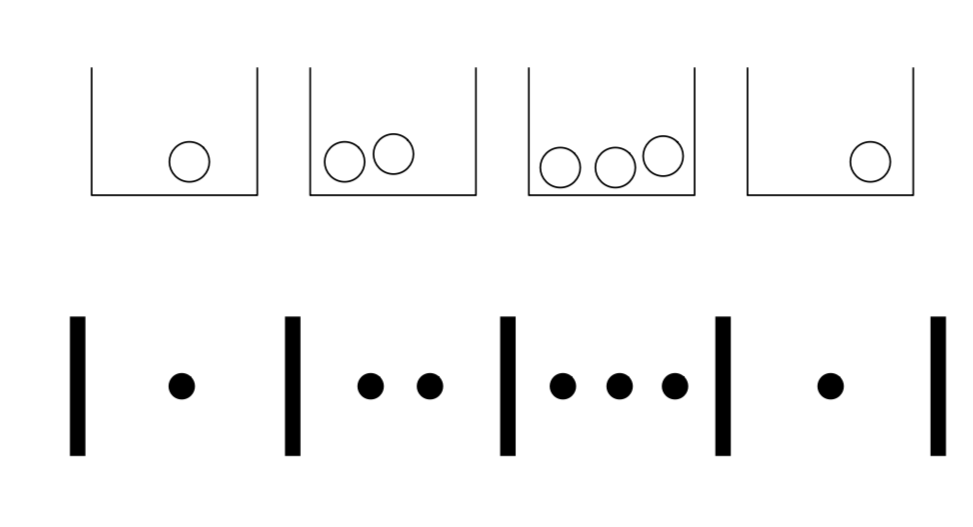
\includegraphics[width=0.4\textwidth]{image/starsandbars.png}
    \end{center}
    Let there be 7 balls and 2 bars be for the physical partitioning into boxes. Since the balls are indistinguishable, all we have to do is count how many ways we can rearrange these 9 objects, which is $\binom{9}{2}=36$.}}
    
    \item Boxes are distinguishable, but balls are indistinguishable, and there needs to be at least one ball in every box.
    
    \medskip 
    \fbox{\parbox{0.9 \textwidth}{
    This is the same, but we fix three balls to be in three boxes, and then do the same analysis as the last problem. Hence, now we have 4 balls that needs to be partitioned into three boxes, so $\binom{6}{2}=15$. }}
    
    \item Neither boxes nor balls are distinguishable. (Hint: just count cases)
    
    \medskip 
    \fbox{\parbox{0.9 \textwidth}{
    If both boxes and balls are indistinguishable, then we have to resort to counting cases.
    \begin{multicols}{2}
    \begin{itemize}
        \item $\{7,0,0\}$
        \item $\{6,1,0\}$
        \item $\{5,2,0\}$
        \item $\{4,3,0\}$
        \item $\{5,1,1\}$
        \item $\{4,2,1\}$
        \item $\{3,2,2\}$
        \item $\{3,1,3\}$
    \end{itemize}
    \end{multicols}
    The general case is very difficult to solve.}}
    
    \item Balls are distinguishable, but boxes are indistinguishable.
    
    \medskip 
    \fbox{\parbox{0.9 \textwidth}{
    If the balls are distinguishable, this is pretty tricky. Based on the casework done in previous section:
    \begin{multicols}{2}
    \begin{itemize}
        \item $\{7,0,0\}$: only 1 way to do this.
        \item $\{6,1,0\}$: $\binom{7}{1}=7$ ways.
        \item $\{5,2,0\}$: $\binom{7}{2}=21$ ways.
        \item $\{4,3,0\}$: $\binom{7}{3}=35$ ways.
        \item $\{4,2,1\}$: $\frac{7!}{4!2!1!}=105$ ways.
        \item $\{5,1,1\}$: $\frac{1}{2}\frac{7!}{5!1!1!}=21$ ways.
        \item $\{3,2,2\}$: $\frac{1}{2}\frac{7!}{3!2!2!}=105$ ways.
        \item $\{1,3,3\}$: $\frac{1}{2}\frac{7!}{3!3!1!}=70$ ways.
    \end{itemize}
    \end{multicols}
    In total we get $1+7+21+35+105+21+105+70=365$ ways. As we can see, the problem gets pretty quickly out of hand!}}
    
\end{enumerate}
\end{prob}

\pagebreak

\begin{prob} 
\begin{enumerate}[label = (\alph*)]

    \item \textbf{(Block-walking problem)} Suppose Mrs. Ant is at position $(0,1)$ on a Cartesian plane. A move consists of $\{\textsc{Up},\textsc{Right}\}$. In how many ways can Mrs. Ant reach Mr. Ant, who is at $(4,6)$ after 9 moves?

    \begin{center}
    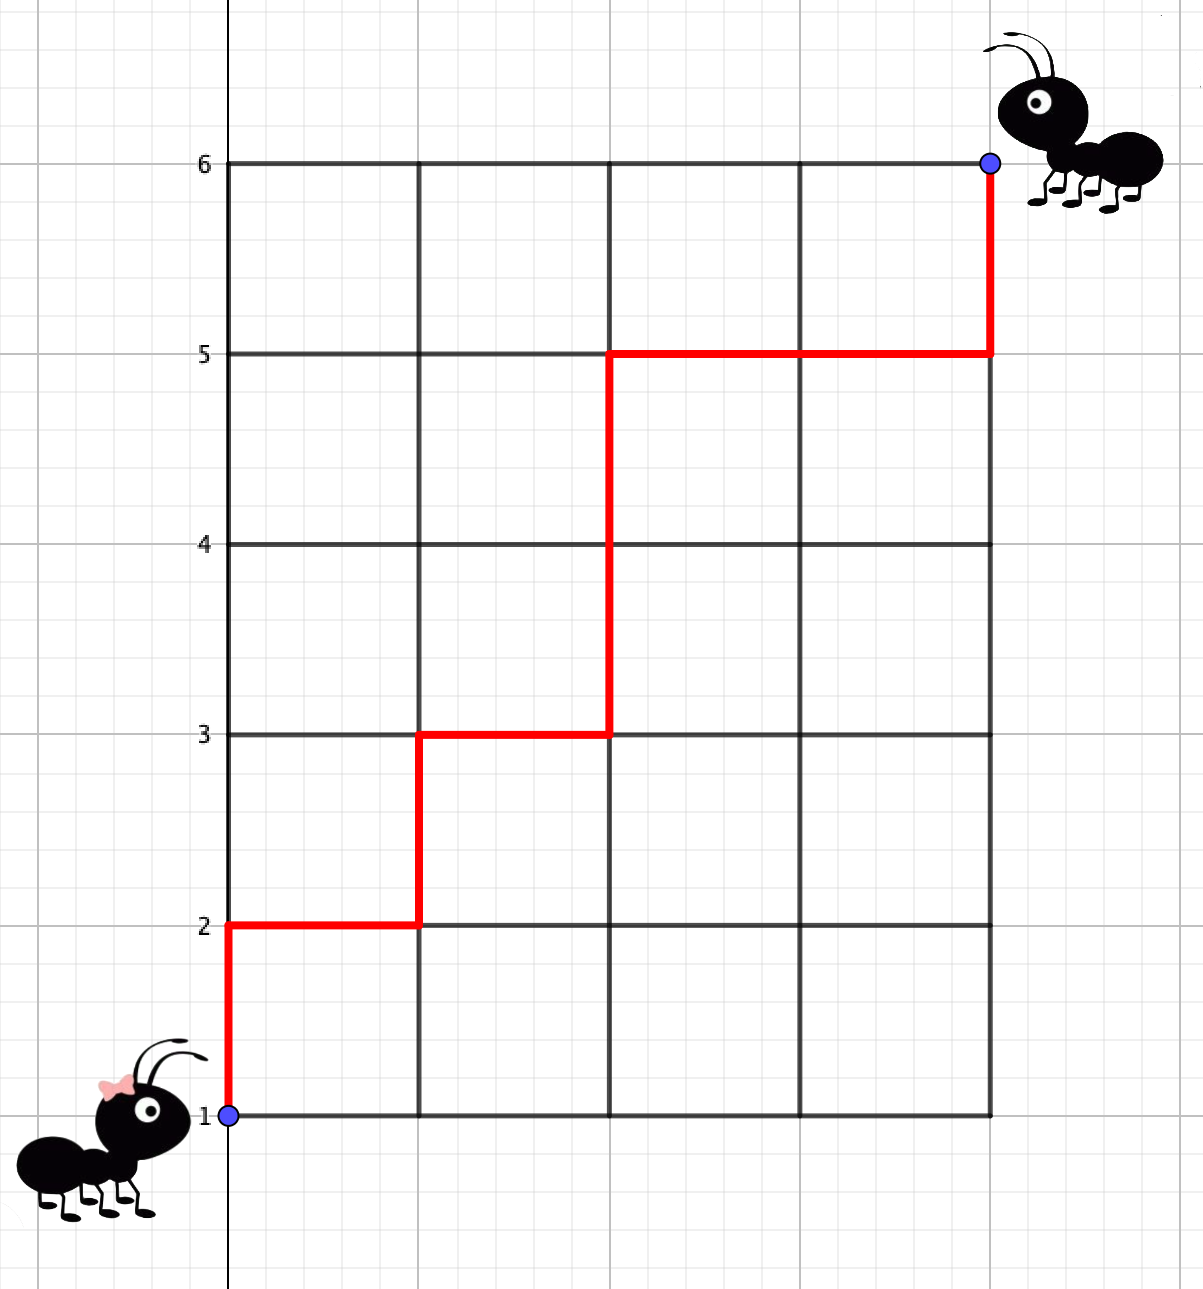
\includegraphics[width=0.6\textwidth]{image/antprob.png}
    \end{center}
    
    \medskip 
    \fbox{\parbox{0.9 \textwidth}{

    A sequence of moves for Mrs. Ant will be, for instance $URURUURRU$ for the illustrated path above. Hence this problems reduces to picking 4 spots for $R$ out of 9 spots, and hence $\binom{9}{4}$.}}
    
    \item \textbf{(A totally different problem, we swear)} A fair die is rolled 4 times. What is the probability that each of the last three rolls is at least as large as the roll preceding it? (i.e. the dice rolls form a sequence of 4 non-decreasing numbers)

    \medskip 
    \fbox{\parbox{0.9 \textwidth}{
    This is in fact, almost as same as the problem above. Let the $i$th dice roll be the coordinate the ant is at after $i$ \textsc{Right} moves. Hence for this path in the illustration, the dice roll would be $2, 3, 5, 5$. The fact that the ant must move up forces the path to trace out dice rolls that forms an increasing sequence. Hence, the probability that this is achieved, using naive definition of probability is: $$ \frac{\binom{9}{4}}{6^4}=\frac{7}{72} $$ Lesson of the problem is: if you see a hard problem, try to redress them into one that you already know! - Credits: 2001 AIME I Problem 6.}}

\end{enumerate}
\end{prob}



\end{document}